\documentclass[11pt,a4paper]{jarticle}
\usepackage[dvipdfmx]{graphicx}
\usepackage{url}
\graphicspath{{./img/eps/}}

\renewcommand{\baselinestretch}{1.05} 
\marginparwidth=0cm
\topmargin=-1cm
\headheight=0.3cm
\headsep=0.7cm
\oddsidemargin=0cm
\evensidemargin=0cm
%\textwidth=43zw
\textwidth=15.92cm
%\textheight=43.3\baselineskip
\baselineskip = 0.5744cm
\textheight=43\baselineskip

\itemsep=0.05\baselineskip
\parsep=0pt
\topsep=0.01\baselineskip
\partopsep=0pt
\listparindent=0zw

%% header and footer
\usepackage{fancyhdr}
\pagestyle{fancy}
\lhead{2018年度 春学期授業}
\chead{インタラクティブ・アート実習}
\rhead{担当教員: 松下 光範}
\cfoot{\thepage}
\renewcommand{\headrulewidth}{0pt}
\renewcommand{\footrulewidth}{0pt}

\usepackage{ascmac}
\usepackage{listings,jlisting}
\usepackage{color}
\definecolor{OliveGreen}{cmyk}{0.64,0,0.95,0.40}
\definecolor{colFunc}{rgb}{1,0.07,0.54}
\definecolor{CadetBlue}{cmyk}{0.62,0.57,0.23,0}
\definecolor{Brown}{cmyk}{0,0.81,1,0.60}
\definecolor{colID}{rgb}{0.63,0.44,0}
\definecolor{rulesepcolor}{gray}{0.666}
\lstset{
  language=Java,%プログラミング言語によって変える。
  basicstyle={\ttfamily\small},
  keywordstyle={\color{OliveGreen}},
  %[2][3]はプログラミング言語によってあったり、なかったり
  keywordstyle={[2]\color{colFunc}},
  keywordstyle={[3]\color{CadetBlue}},%
  commentstyle={\color{Brown}},
  %identifierstyle={\color{colID}},
  stringstyle=\color{blue},
  tabsize=2,
  %frame=trBL,
  %numbers=left,
  numberstyle={\ttfamily\small},
  breaklines=true,%折り返し
  %backgroundcolor={\color[gray]{.95}},
  framexleftmargin=0mm,
  frame=single,
  rulesepcolor=\color{rulesepcolor},
  captionpos=b
}


%%%%%%%%%%%%%%%%%%%%%%%%%%%%%%%%%%%%%%%%%%%%%%%%%%%%%%%%%%%%%%%%
\begin{document}

% title
\section*{\LARGE{第2講 プログラミングでLEDを制御する}}
\section{本実習の目標}
\begin{itemize}
\item Processing で図形や絵を描いてみる
\item Processing に Arduino (Firmata) をインストールする
\item Processing から Arduino を制御するためのシリアルポートを把握する
\item Arduino の Digital Output を用いてLEDを光らせる
\item Arduino の Digital Input を用いてスイッチの ON/OFF を取得する
\end{itemize}

%%%%%%%%%%%%%%%%%%%%%%%%%%%%%%%%%%%%%%%%%%%%%%%%%%%%%%%%%%%%%%%%


\section{Processing の基礎}
本実習では Processing\footnote{\url{http://processing.org}} というプログラミング言語を用います。
Processing は、Java を単純化し、グラフィック機能に特化した言語です。

Processing による基本的なプログラミングを行います。
なお、メニューバーの Help → Reference でインターネットブラウザが起動し、より詳しい説明が確認できますので、そちらも参考にしてください。
ただし英語表記です。
Processing にはあらかじめサンプルコード(お手本になるプログラム)が、たくさん用意されているので、それを動かしてみてどんなことができるかを見ておくのも良いかもしれません。
サンプルコードは、メニューバーの File → Example から見ることができます。

\begin{figure}[h!]
 \centering
 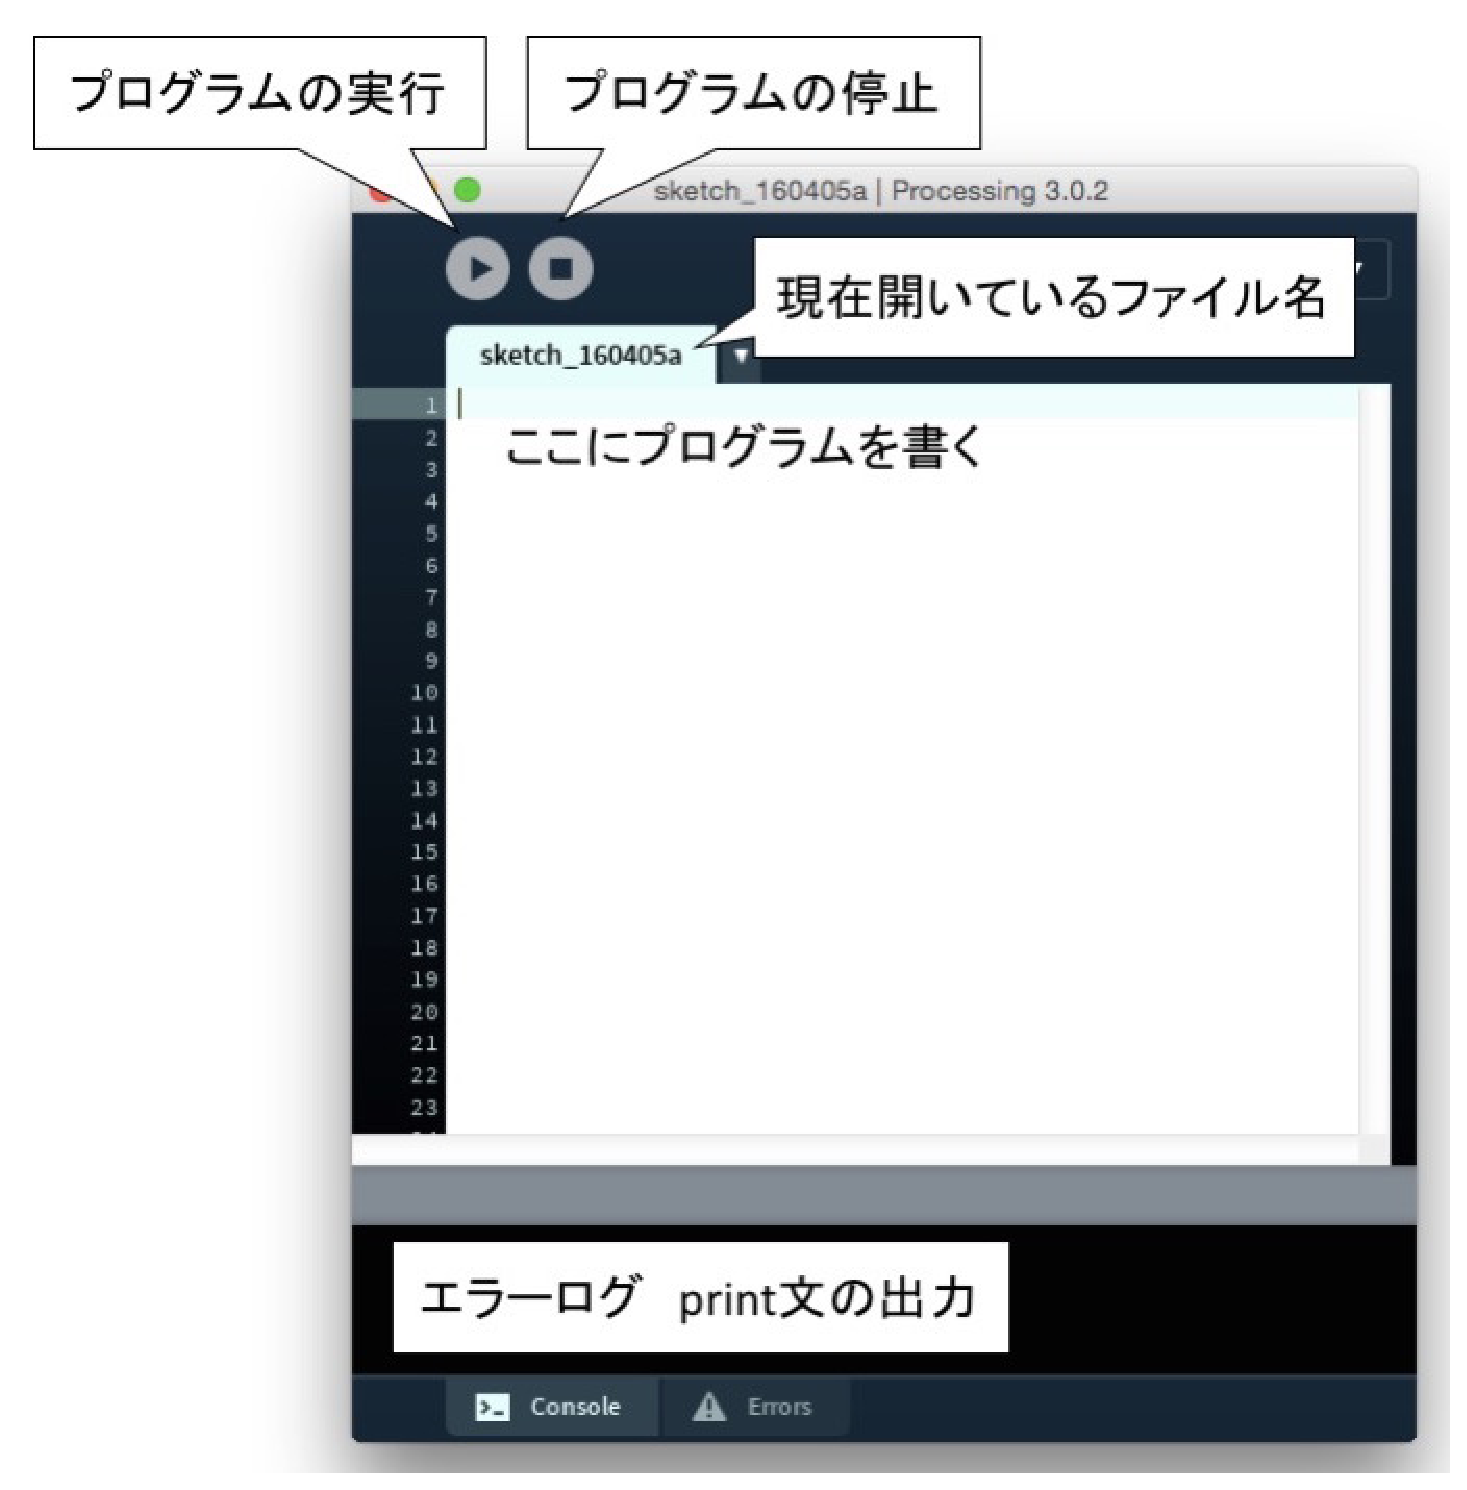
\includegraphics[width=0.35\columnwidth]{processing_ide.eps}
 % \caption{Processing の IDE (統合開発環境)}
\end{figure}

\subsection*{基本的な図形を描く}

\begin{itemize}
 \item \textbf{四角形を書く}: rect(x, y, w, h);

       x = x座標、
       y = y座標、
       w = 四角形の幅、
       h = 四角形の高さ

\begin{figure}[htbp]
 \begin{minipage}{0.325\hsize}
  \begin{center}
   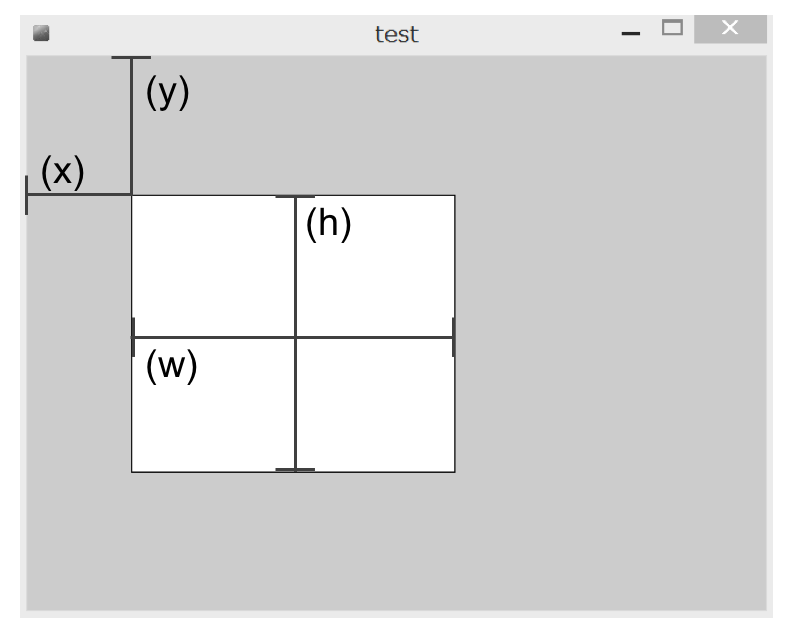
\includegraphics[width=40mm]{image_of_rect_function.eps}
  \end{center}
 \end{minipage}
 \begin{minipage}{0.325\hsize}
 \begin{center}
  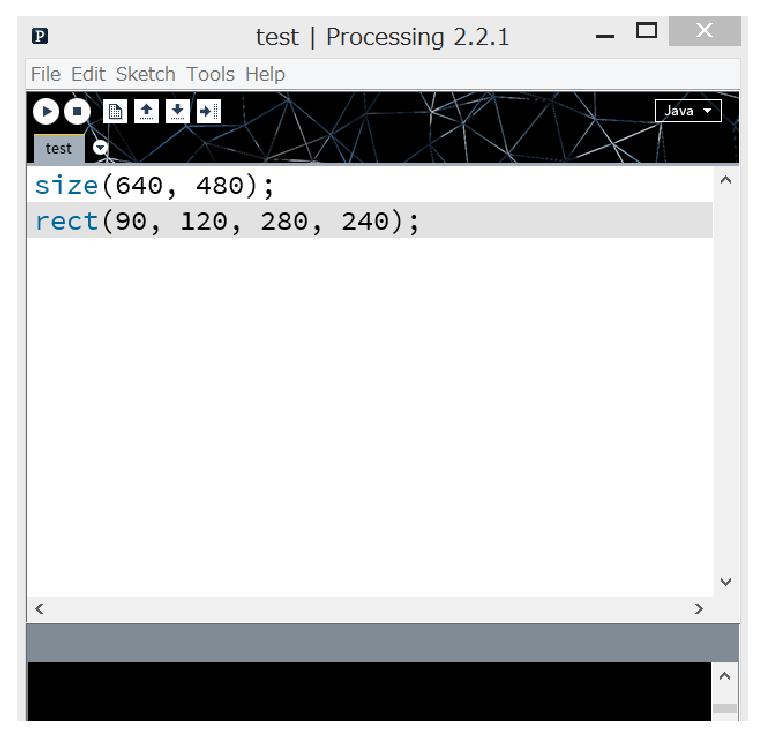
\includegraphics[width=40mm]{Processing_img1-1.eps}
 \end{center}
 \end{minipage}
 \begin{minipage}{0.325\hsize}
 \begin{center}
  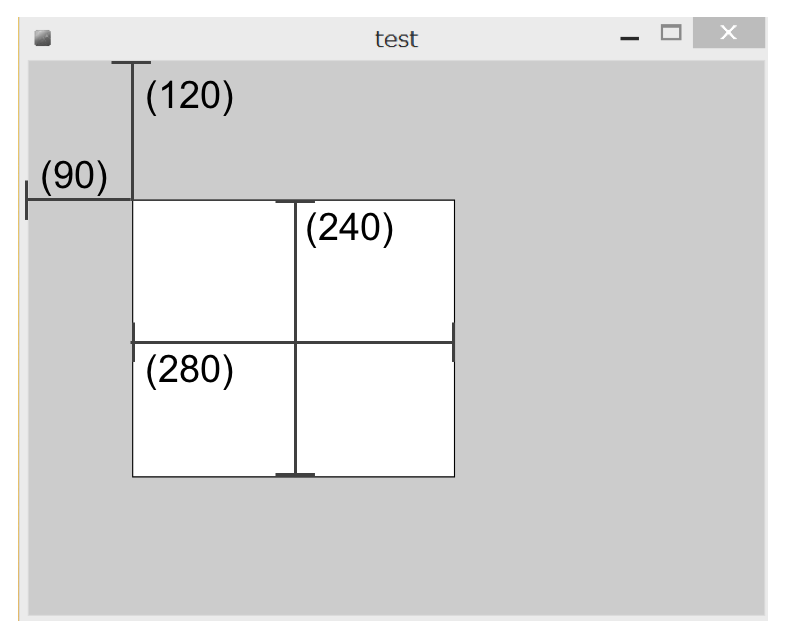
\includegraphics[width=40mm]{example_of_rect_function.eps}
 \end{center}
 \end{minipage}
\end{figure}

 \item \textbf{円を書く}: ellipse(x, y, w, h);

\begin{figure}[htbp]
 \begin{minipage}{0.5\hsize}
  \begin{center}
   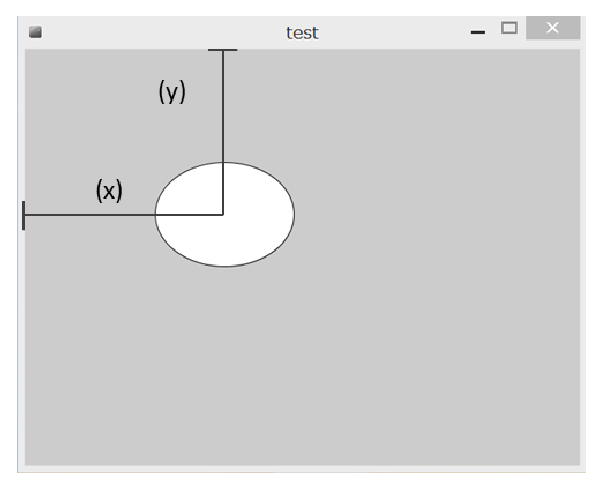
\includegraphics[width=40mm]{Processing_img1-6.eps}
  \end{center}
 \end{minipage}
 \begin{minipage}{0.5\hsize}
 \begin{center}
  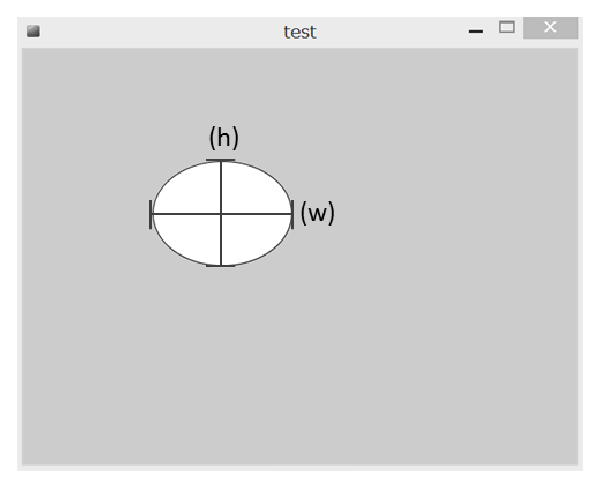
\includegraphics[width=40mm]{Processing_img1-8.eps}
 \end{center}
 \end{minipage}
\end{figure}

\begin{figure}[htbp]
 \begin{minipage}{0.325\hsize}
  \begin{center}
   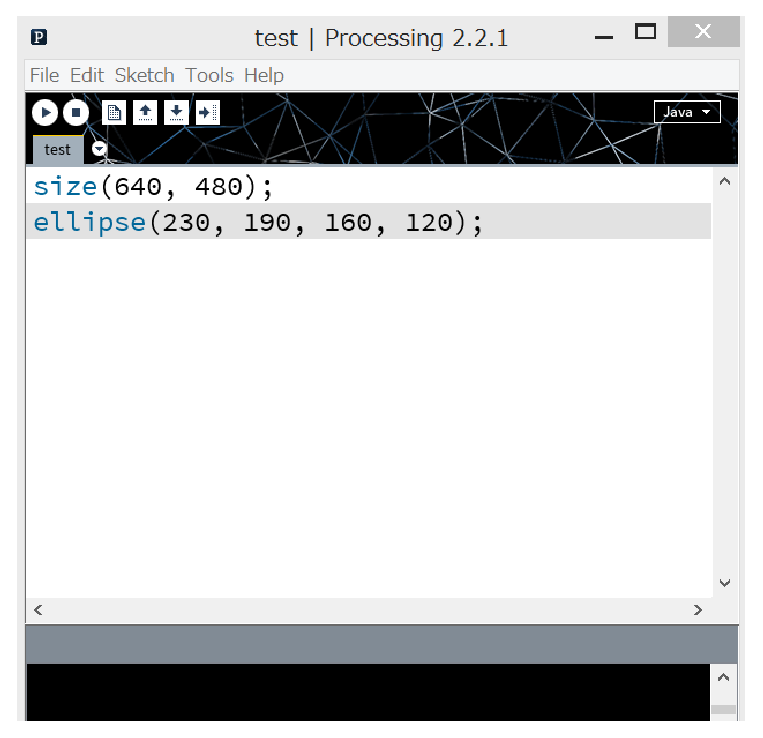
\includegraphics[width=40mm]{Processing_img1-4.eps}
  \end{center}
 \end{minipage}
 \begin{minipage}{0.325\hsize}
 \begin{center}
  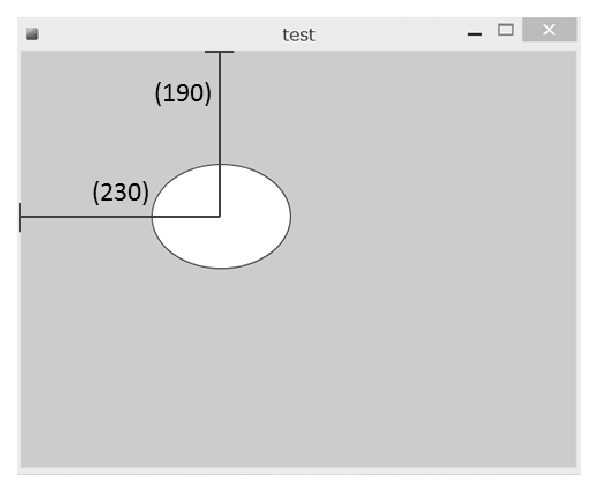
\includegraphics[width=40mm]{Processing_img1-5.eps}
 \end{center}
 \end{minipage}
 \begin{minipage}{0.325\hsize}
 \begin{center}
  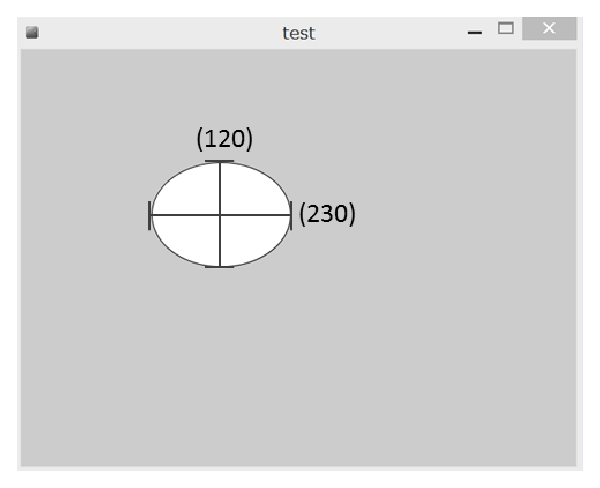
\includegraphics[width=40mm]{Processing_img1-7.eps}
 \end{center}
 \end{minipage}
\end{figure}

 \item \textbf{線を書く}: line(x1, y1, x2, y2);
       
       x1 = 始点のx座標、
       y1 = 始点のy座標、
       x2 = 終点のx座標、
       y2 = 終点のy座標

 % \item \textbf{三角形を書く}: triangle(x1, y1, x2, y2, x3, y3);
\end{itemize}


\subsection*{図形の色を変える}
% \begin{tabular}{lll}
%  \textbf{図形の色を変える:} & fill(r, g, b); & r, g, b をそれぞれ 256 段階で指定 \\
%  \textbf{図形の色を消す:} & noFill(); &  \\ 
%  \textbf{線の色を変える:} & stroke(r, g, b); &  \\ 
%  \textbf{線の色を消す:} & noStroke(); &  \\ 
%  % \textbf{線の幅を指定する:} & strokeWeight(weight); & weight = 線の太さ \\ 
%  \textbf{ウィンドウの背景色を変える:} & background(r, g, b); &  \\ 
% \end{tabular}
Processing で図形などの色を指定したいときは、Red、Green、Blue をそれぞれ 256 段階で指定します。
\begin{lstlisting}
 // 四角形を赤で表示する
 fill(255, 0, 0);        // 赤は r = 255, g = 0, b = 0
 rect(10, 10, 100, 50);
\end{lstlisting}
また、グレースケールで指定する方法もあります。
\begin{lstlisting}
 fill(0);               // 0 (黒) から 255 (白) で指定
\end{lstlisting}
白から黒の色で指定したいときはこちらの方が楽です。

\begin{itemize}
 \item \textbf{図形の色を変える}: fill(r, g, b);
 \item \textbf{図形の色を消す}: noFill();
 \item \textbf{線に色をつける}: stroke(r, g, b);
 \item \textbf{線の色を消す}: noStroke();
 \item \textbf{ウィンドウの背景色を変える}: background(r, g, b);
\end{itemize}


\subsection*{初期化とループ処理}
Processing では、プログラムを実行時に setup 関数が 1 度実行され (初期化) 、その後 draw関数 が繰り返されます (ループ処理)。
setup と draw を用いるとアニメーションなどの動的な表現ができます。

\begin{lstlisting}
 void setup(){
   // 初期化の処理をここに書く
   // プログラム開始時に1度だけ実行される
   // size(w, h); などはここへ
 }

 void draw(){
   // 繰り返したい処理をここに書く
   // setup()が実行された後にプログラムが終了するまで繰り返される
 }
\end{lstlisting}

\newcounter{nombre}
\setcounter{nombre}{1}
\subsection*{TRY\thenombre: Processing でベースとなるプログラムを作成する}
\label{Base}
\refstepcounter{nombre}

\begin{enumerate}
 \item ウィンドウサイズを幅 300 pixel、高さ 300 pixel に
 \item ウィンドウの背景色を黒に
 \item 幅 100 pixel、幅 100 pixel の円を青色で表示
\end{enumerate}

\begin{lstlisting}
 void setup() {
   size(???, ???);
 }

 void draw() {
   background(???, ???, ???);

   fill(???, ???, ???);
   ellipse(???, ???, ??? ???);
 }
\end{lstlisting}

\subsection*{TRY\thenombre: マウスボタンがクリックされたら図形を表示する}
\label{mousePressed}
\refstepcounter{nombre}

%%TRY\ref{Base} %%なぜかこれで1にならない...
TRY1で作ったプログラムを改造し、マウスが押されたときにウィンドウに図形が表示されるようにします。

Processing では、あらかじめ用意されている「mousePressed」という変数を用いることで、マウスのクリック動作を簡単に検出することができます。
\begin{lstlisting}
 if (mousePressed) {
   // マウスボタンを押したときの処理
 } else {
   // マウスボタンを押していないときの処理
 }
\end{lstlisting}


\subsection*{TRY\thenombre: マウスポインタで図形を操作する}
\refstepcounter{nombre}

TRY\ref{mousePressed} で作ったプログラムを改造し、マウスポインタの位置に合わせて図形が表示されるようにします。

Processing では、あらかじめ用意されている「mouseX」「mouseY」という変数を用いることで、マウスポインタの x 座標と y 座標を取得できます。


\begin{lstlisting}
 void setup() {
   size(300, 300);
 }

 void draw() {
   if (mousePressed) {
      ellipse(mouseX, mouseY, 32, 32);
   }
 }
\end{lstlisting}



\section{Arduino の準備}
まず、Processing から Arduino を用いるための準備をしましょう。
本実習ではスイッチやセンサ、LED などを PC から制御するために Arduino\footnote{\url{http://arduino.cc}} というマイコンを用います。

本来、Arduino と Processing を連携させるためには、シリアル通信を用いますが、そのためのプログラムを書くのは少し面倒です。
実習では楽をするために、Firmata\footnote{\url{http://firmata.org}} を用います。

\subsection*{★ライブラリのインストール方法}
%Firmataを用いるにあたって、ライブラリをインストールしなければなりません。

まず、ライブラリをインストールするためにWiFiに接続します。
%%画像入れる
\begin{figure}[htbp]
  \centering
  \includegraphics[width=0.75\columnwidth]{img/eps/WiFi.eps}
%  \caption{}
\end{figure}

Processingのメニューから以下のライブラリを追加します。
\begin{itemize}
\item スケッチ → ライブラリをインポート... → ライブラリを追加...
\end{itemize}

\begin{figure}[htbp]
  \centering
  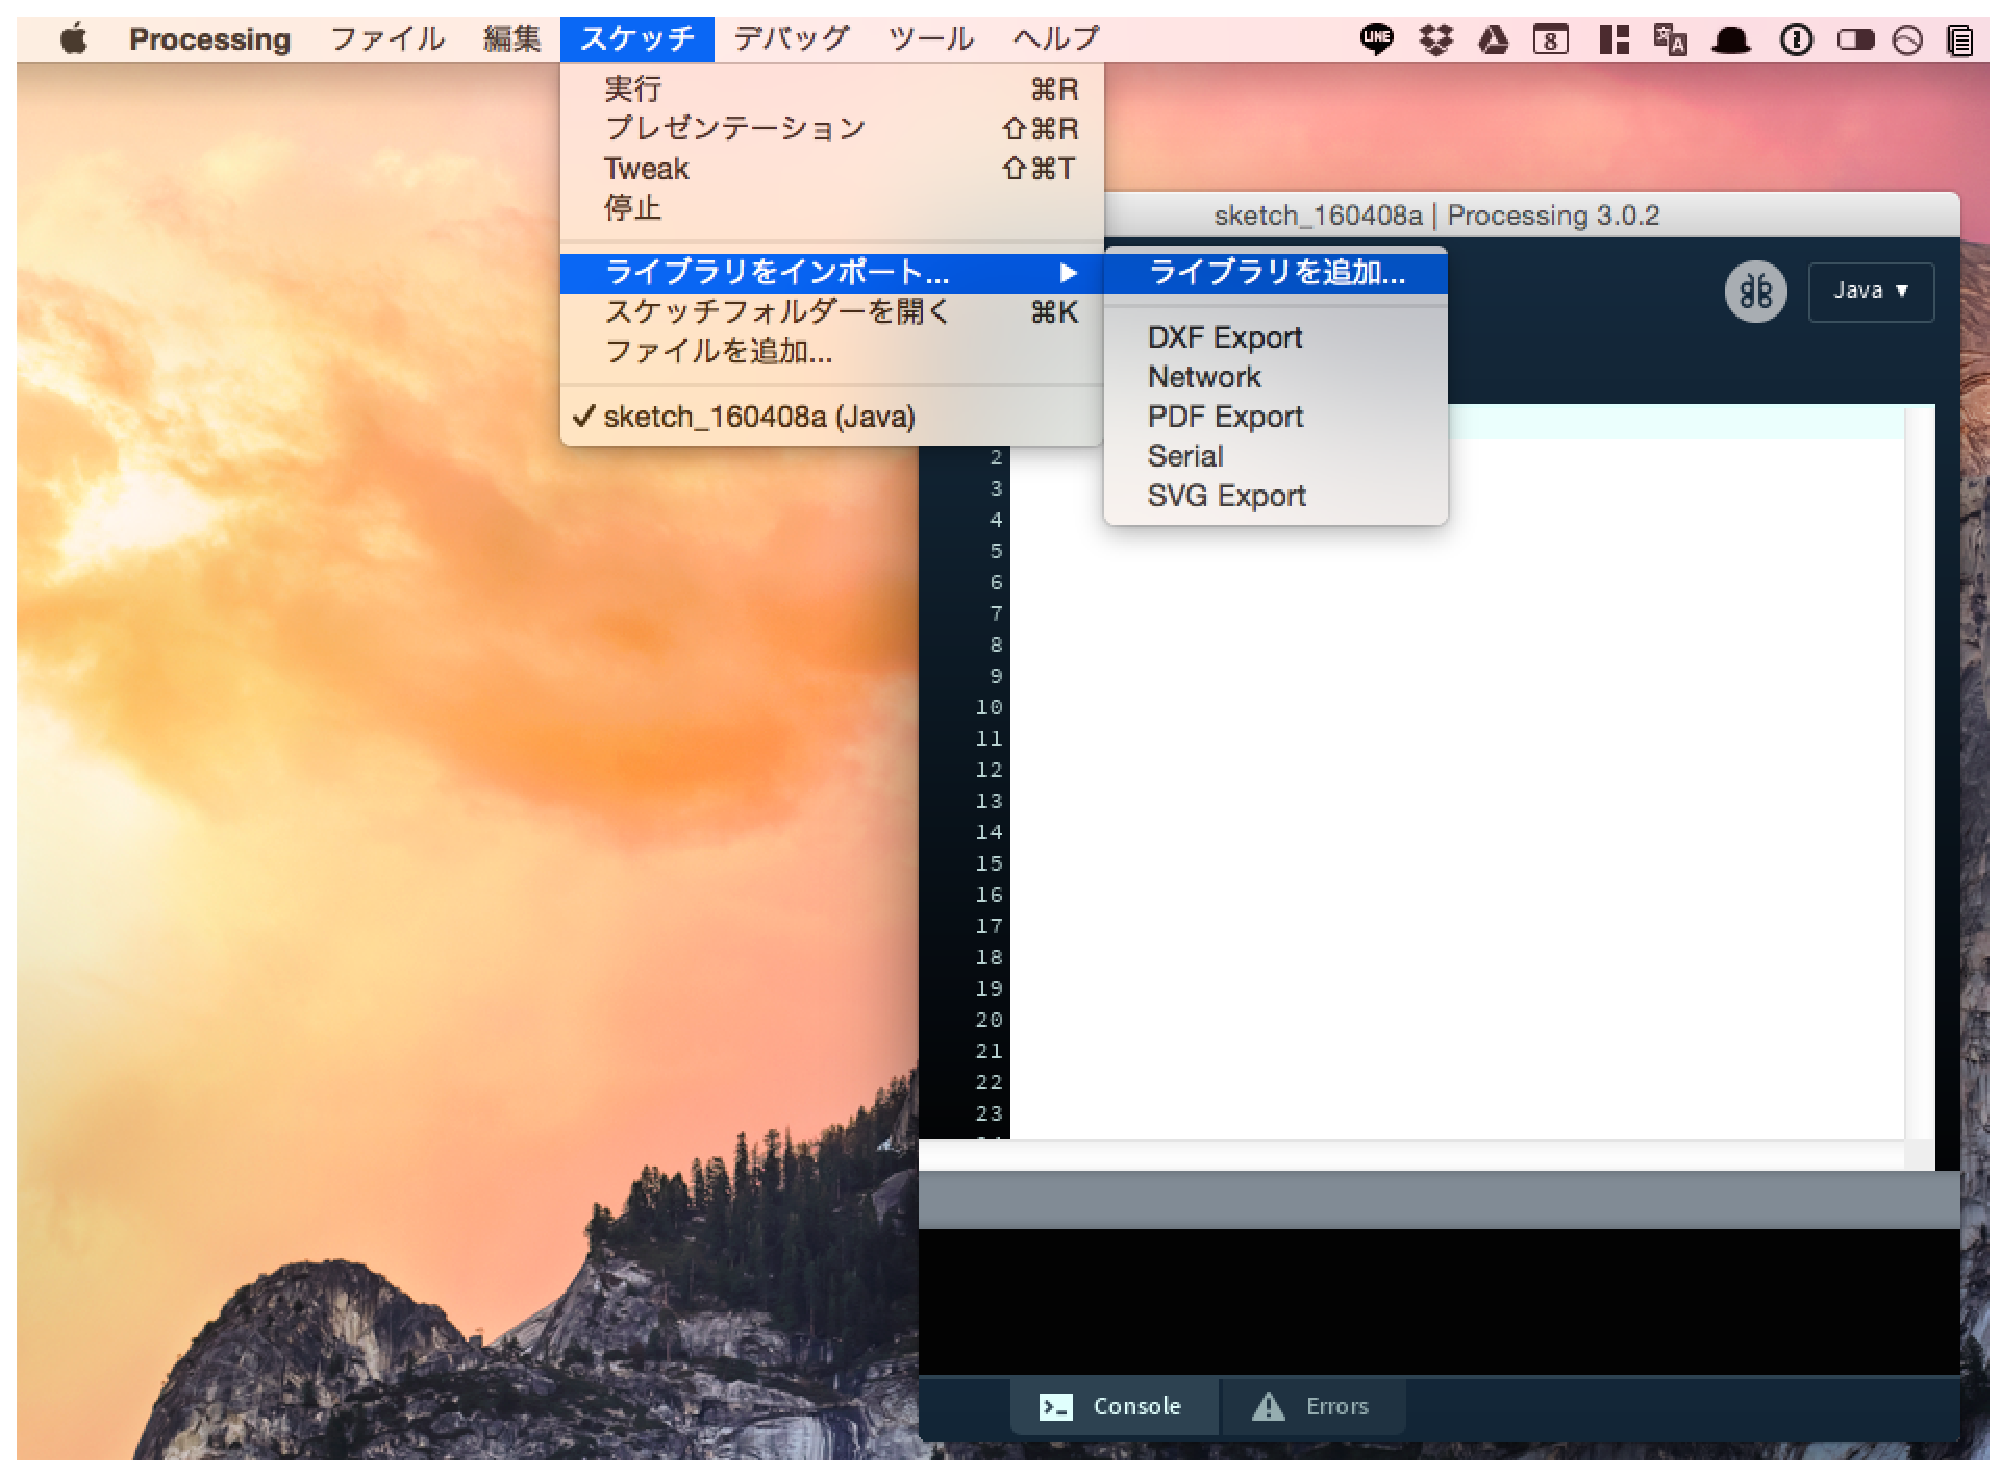
\includegraphics[width=0.75\columnwidth]{img/eps/how_to_install_the_Firmata_library1.eps}
%  \caption{}
  \label{figure:LED}
\end{figure}

\newpage

\begin{itemize}
\item 図2のように検索バーで「firmata」と入力し、「Arduino(Firmata)」を選択、「Install」をクリックします。
\end{itemize}

\begin{figure}[htbp]
  \centering
  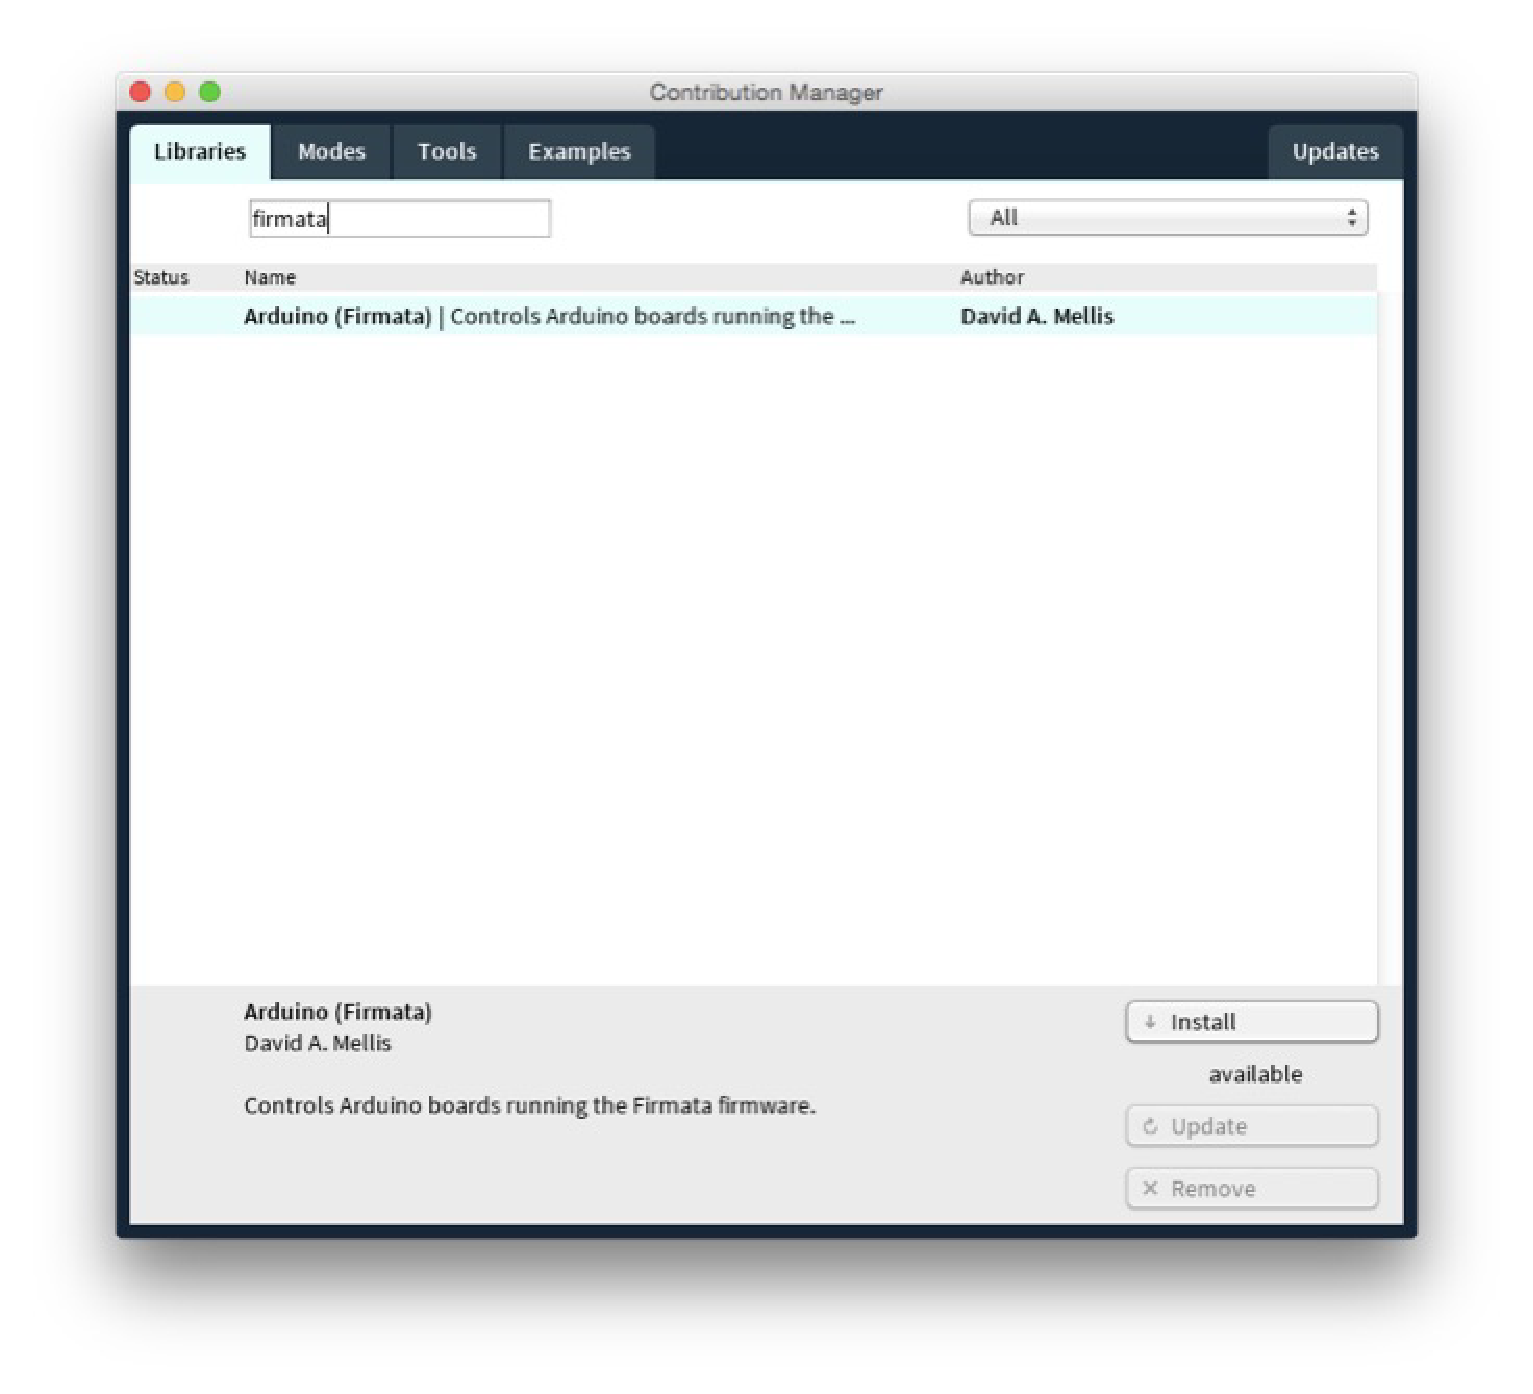
\includegraphics[width=0.6\columnwidth]{img/eps/how_to_install_the_Firmata_library2.eps}
  %\caption{ライブラリ選択画面}
  \label{figure:switch}
\end{figure}

これでライブラリのインストールは完了です。

%\begin{figure}[h!]
 %\begin{minipage}{0.5\columnwidth}
  %\centering
  %\includegraphics[width=0.9\columnwidth]{img/library01.eps}
 %\end{minipage}
 %\begin{minipage}{0.5\columnwidth}
  %\centering
  %\includegraphics[width=0.9\columnwidth]{img/library02.eps}
 %\end{minipage}
  %\caption{プルアップ抵抗 (左) とプルダウン抵抗 (右)}
%\end{figure}


%\subsection*{Todo}
%\begin{itemize}
% \item Processing に Arduino ライブラリをインストール       
% \item 動作確認
%\end{itemize}

%まず、Processing から Arduino を用いるための準備をしましょう。
%Arduino の Digital Output を用いて LED を制御する。Digital Input を用いてスイッチの ON/OFF を取得する。

\newpage

\section{シリアルポートの確認}
ProcessingからArduinoにインストールしたFirmataを操作するには、使用しているシリアルポートの環境を知る必要があります。まず、下記のコードをProcessingに入力してください。
\begin{lstlisting}
import processing.serial.*;
import cc.arduino.*;
Arduino arduino;
 
void setup() {
  println(Arduino.list());
}
\end{lstlisting}
すると、Processingの下部のコンソールに以下のようなメッセージが表示されます。
%コンソールのメッセージ%
\begin{lstlisting}
/dev/cu.Bluetooth-Incoming-Port
/dev/cu.Bluetooth-Modem
/dev/cu.usbmodem1421
/dev/tty.Bluetooth-Incoming-Port
/dev/tty.Bluetooth-Modem
/dev/tty.usbmodem1421
\end{lstlisting}
次に、「/dev/...」から始まる記述に対して、それぞれ順番に0から番号を付与します。
\begin{lstlisting}
[0] /dev/cu.Bluetooth-Incoming-Port
[1] /dev/cu.Bluetooth-Modem
[2] /dev/cu.usbmodem1421
[3] /dev/tty.Bluetooth-Incoming-Port
[4] /dev/tty.Bluetooth-Modem
[5] /dev/tty.usbmodem1421
\end{lstlisting}
この中から、「/dev/tty.usbmodem…」もしくは「/dev/tty.usbserial…」から始まる記述の番号 (上記の例では5番) をメモしておいてください。
Arduino を使うためにはシリアルポートの指定をしなければなりません。
続いて、下記のコードのArduino.list()[5] の部分の数字を先ほどメモした番号に変更し、Processingに入力してください。
\begin{lstlisting}
 import processing.serial.*;
 import cc.arduino.*;

 Arduino arduino;

 void setup() {
   // Arduino の初期化
   // シリアルポートの指定など
   // Arduino.list()[5] は環境によって変える
   arduino = new Arduino(this, Arduino.list()[5], 57600);
 }
\end{lstlisting}

これで Processing から Arduino を用いるための準備は完了です。これらの命令は今後も Arduino を用いる際に必ず使うので、テンプレートとして保存しておきましょう。

\begin{itemize}
\item ファイル → 名前を付けて保存... → 「ArduinoTemplate」という名前で保存します。
\end{itemize}

今後、Arduinoを使用するプログラムを書く際は、この「ArduinoTemplate」をもとに編集しましょう。


\newpage

\section{Digital Output}
では、まず簡単なプログラムで動作を確認してみましょう。LEDが点灯するプログラムを作成してみましょう。Arduino側は、Digital Outの13番にLEDを接続しておきます。

\subsection{LED を点灯させる}
Digital Output を使って LED を点灯させてみましょう。

\subsubsection*{回路}
\begin{figure}[h!]
 \begin{minipage}{0.5\columnwidth}
  LED を接続したピンに電圧をかけると LED が点灯する回路を作りましょう。
  \begin{itemize}
   \item \textbf{使う部品}
	 \begin{itemize}
	  \item Arduino
	  \item 抵抗
	  \item LED
	 \end{itemize}
   \item \textbf{ポイント}
	 \begin{itemize}
	  \item 5V → LED → 抵抗 → GND の順に
	  \item LED には極性があるので向きに注意
	 \end{itemize}
  \end{itemize}
 \end{minipage}
 \begin{minipage}{0.5\columnwidth}
  \centering
  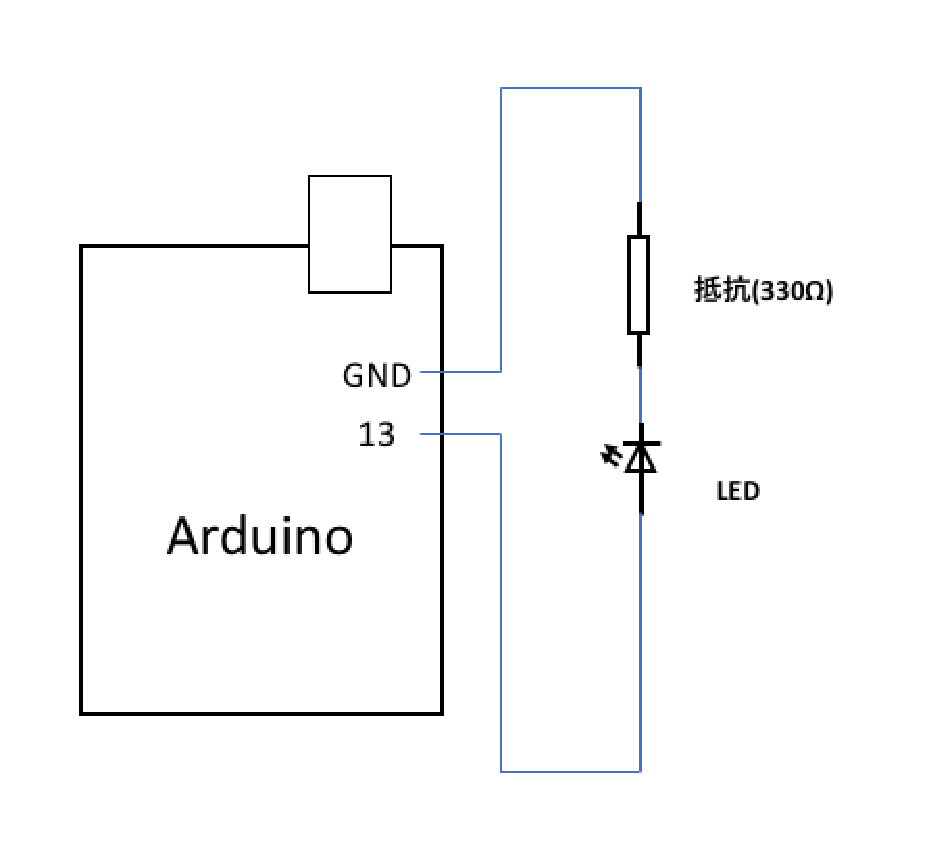
\includegraphics[width=80mm]{img/eps/kairo2.eps}
  \caption{回路図}
 \end{minipage}
\end{figure}

\subsubsection*{プログラム}
\begin{lstlisting}
import processing.serial.*;
import cc.arduino.*;
 
Arduino arduino;
int ledPin = 13; // LED を接続したピンの番号
 
void setup() {
  arduino = new Arduino(this, Arduino.list()[5], 57600);

  // Arduino のピンモードを設定
  // ここでは 13 番ピンを Output 用に設定
  arduino.pinMode(ledPin, Arduino.OUTPUT);
}
 
void draw() {
  // Arduino の 13 番ピンを HIGH (5V) に
  arduino.digitalWrite(ledPin, Arduino.HIGH);
}
\end{lstlisting}

\subsection{LED を点滅させる}
Digital Output を使って LED を点滅させてみましょう。

\subsubsection*{プログラム}
\begin{lstlisting}
import processing.serial.*;
import cc.arduino.*;
 
Arduino arduino;
int ledPin = 13; // LED を接続したピンの番号
 
void setup() {
  arduino = new Arduino(this, Arduino.list()[5], 57600);

  // Arduino のピンモードを設定
  // ここでは 13 番ピンを Output 用に設定
  arduino.pinMode(ledPin, Arduino.OUTPUT);
}
 
void draw() {
  // Arduino の 13 番ピンを HIGH (5V) に
  arduino.digitalWrite(ledPin, Arduino.HIGH);
  delay(500); // 500ミリ秒間待つ

  // Arduino の 13 番ピンを LOW (0V) に
  arduino.digitalWrite(ledPin, Arduino.LOW);
  delay(500);
}
\end{lstlisting}

\subsection{Processingの入力に応じてLEDを点灯させる}
Processingの画面上でマウスを押すとLEDが点灯するプログラムを作成してみましょう。Arduino側は、Digital Outの13番にLEDを接続しておきます。

\subsection*{mousePressed}
mousePressed 変数はマウスが押されているか押されていないかによって、それぞれ true と false に値が変わります。
これを用いると、「マウスがクリックされたときに何かをする」という動作が実現できます。

\begin{lstlisting}
 if (mousePressed) {
   // マウスが押されているときの処理
 } else {
   // マウスが押されていないときの処理
 }
\end{lstlisting}

\subsubsection*{プログラム}
\begin{lstlisting}
import processing.serial.*;
import cc.arduino.*;
 
Arduino arduino;
int ledPin = 13;
color bgColor = color(0);
 
void setup() {
  size(400, 200);
  arduino = new Arduino(this, Arduino.list()[5], 57600);
  arduino.pinMode(ledPin, Arduino.OUTPUT);
}
 
void draw() {
  if (mousePressed) {
    arduino.digitalWrite(ledPin, Arduino.HIGH);
    bgColor = color(255,0,0);
  }else{
    arduino.digitalWrite(ledPin, Arduino.LOW);
    bgColor = color(0);
  }
  background(bgColor);
}
\end{lstlisting}
画面をクリックすると、LEDが点灯します。

\section{Digital Input}
\subsection{スイッチの ON/OFF を読み取る}
Arduino の Digital Input を用いてスイッチの ON/OFF を取得する。

\subsubsection*{回路}
デジタル回路の場合、入力端子がどこにも接続されていないような状態 (オープン) が起こると、電圧が High または Low に定まらず誤動作の原因になります。
そのため、回路を安定させるためにプルアップ抵抗/プルダウン抵抗と呼ばれる抵抗を用います。

\begin{figure}[h!]
 \begin{minipage}{0.5\columnwidth}
  \centering
  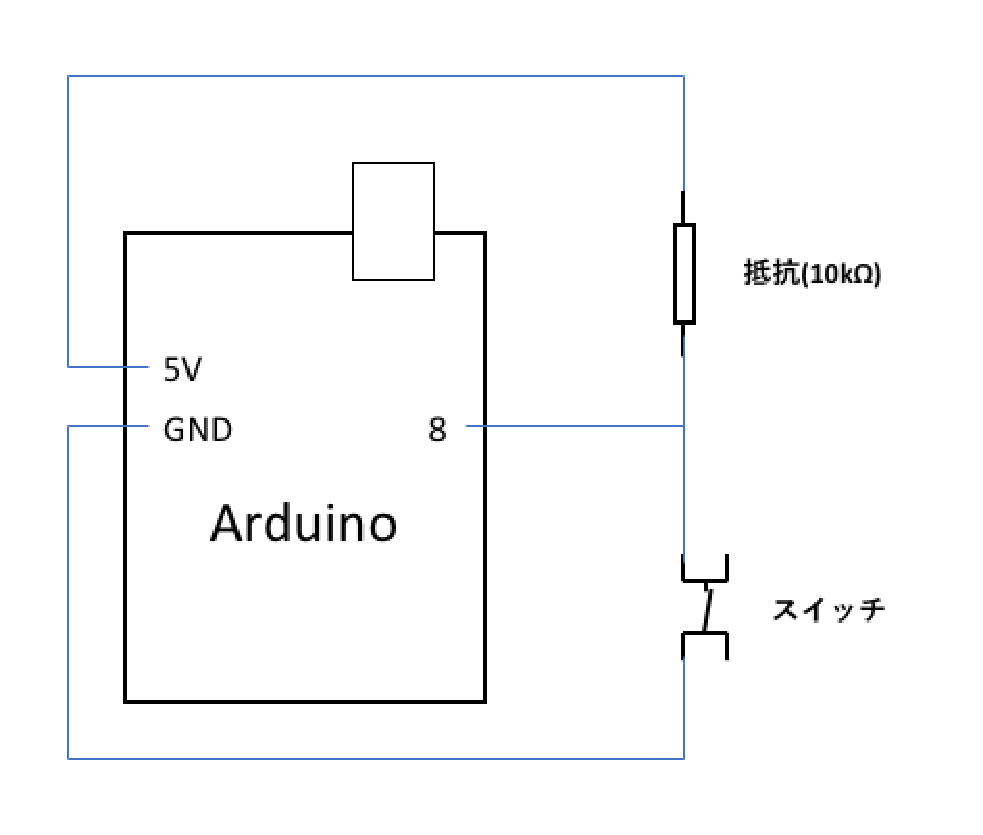
\includegraphics[width=0.7\columnwidth]{img/eps/pull_up.eps}
 \end{minipage}
 \begin{minipage}{0.5\columnwidth}
  \centering
  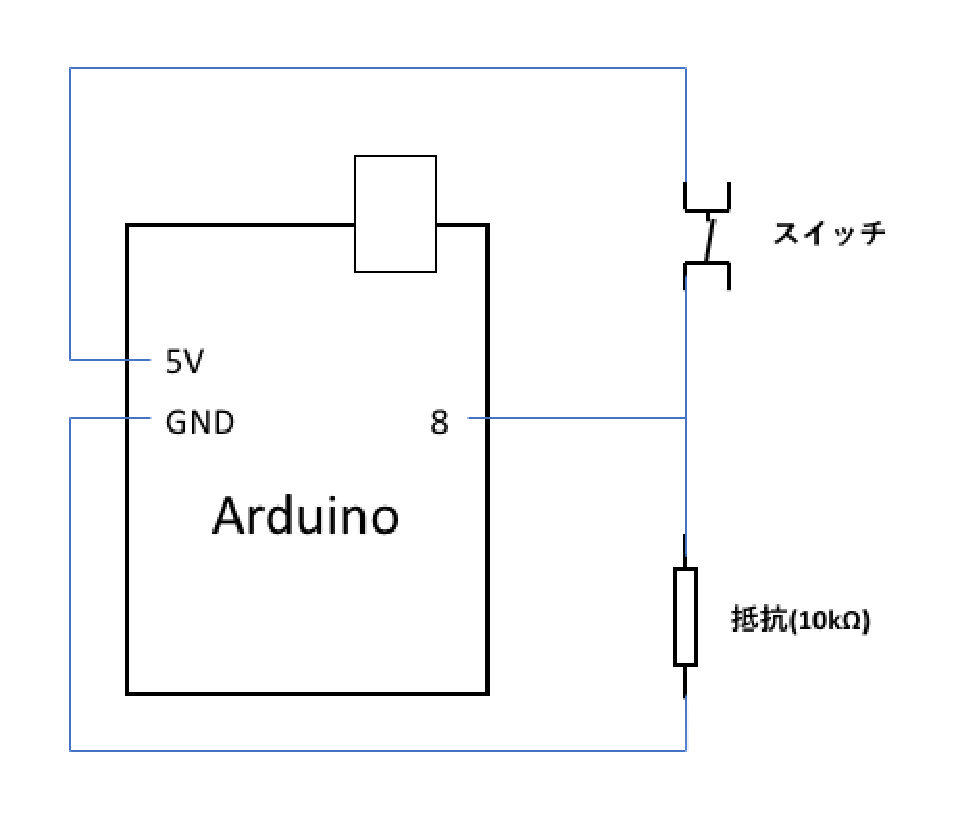
\includegraphics[width=0.7\columnwidth]{img/eps/pull_down.eps}
 \end{minipage}
  \caption{プルアップ抵抗 (左) とプルダウン抵抗 (右)}
\end{figure}

\newpage

\subsubsection*{プログラム}
\begin{lstlisting}
import processing.serial.*;
import cc.arduino.*;

Arduino arduino;
int switchPin = 8; // スイッチを接続したピンの番号
 
void setup() {
  size(400, 300);
  arduino = new Arduino(this, Arduino.list()[5], 57600);
  arduino.pinMode(switchPin, Arduino.INPUT); // ピンモードを Input に
}
 
void draw() {
  // 8 番ピンの電圧を取得し、それが HIGH ならば
  if (arduino.digitalRead(switchPin) == Arduino.HIGH) {
    background(255, 0, 0); // 背景を赤に
  } else {
    background(0, 0, 0);   // そうでなければ (LOW ならば) 背景を黒に
  }
}
\end{lstlisting}


%\subsection*{スイッチを押すと LED が点灯するようにする}
%スイッチの入力を Processing で取得し、それに基づいて LED を制御しましょう。
%上 2 つの合わせ技です。

%これで入力と出力の両方が実現できるようになります。
%次回以降の実習でも入力や出力のための部品が変わるだけで基本的な考え方は同じです。


%\subsubsection*{TRY}
%今回やったことを思い出しながら、回路とプログラムを作成してみましょう。

% \subsubsection*{プログラムを書く}
% \begin{lstlisting}
% import processing.serial.*;
% import cc.arduino.*;

% Arduino arduino;
% int ledPin = 13;
% int switchPin = 8;
 
% void setup() {
%   size(400, 300);
%   arduino = new Arduino(this, Arduino.list()[0], 57600);
%   arduino.pinMode(switchPin, Arduino.INPUT);
%   arduino.pinMode(ledPin, Arduino.OUTPUT);
% }
 
% void draw() {
%   if (arduino.digitalRead(switchPin) == Arduino.HIGH) {
%     background(255, 0, 0);
%     arduino.digitalWrite(ledPin, Arduino.HIGH);
%   } else {
%     background(0, 0, 0);
%     arduino.digitalWrite(ledPin, Arduino.LOW);
%   }
% }
% \end{lstlisting}

\end{document}
